\documentclass[a4paper,12pt,twoside]{article}

\usepackage{graphicx}
\usepackage{amsmath}
\usepackage[english]{babel}
\usepackage[utf8]{inputenc}
\usepackage[colorlinks,bookmarks=false,linkcolor=blue,urlcolor=blue]{hyperref}
\usepackage{color}
\usepackage[T1]{fontenc}
\usepackage{float}
\usepackage{url}
\usepackage{lscape}
\usepackage{tikz}
\usetikzlibrary{patterns,decorations.pathreplacing}
\usepackage[stable]{footmisc}
\usepackage{wrapfig}
\usepackage{textcomp}
\usepackage{changepage}
\usepackage{booktabs}
\usepackage{subfig}
\usepackage{amssymb}
\usepackage[section]{placeins}
\usepackage{mathabx}


\paperheight=297mm
\paperwidth=210mm

\setlength{\textheight}{235mm}
\setlength{\topmargin}{-1.2cm} 
\setlength{\textwidth}{15cm}
\setlength{\oddsidemargin}{0.56cm}
\setlength{\evensidemargin}{0.56cm}

\pagestyle{plain}

% def
\def \be {\begin{equation}}
\def \ee {\end{equation}}
\def \dd  {{\rm d}}
\def \bf {\textbf}
\def \bea {\begin{eqnarray}}
\def \eea {\end{eqnarray}}
\def \bi {\begin{itemize}}
\def \ei {\end{itemize}}
\def \ib {\item[$\bullet$]}
\def \H {{\mathcal H}}
\def \grad{\nabla}
\def \( {\left(}
\def \) {\right)}
\def \order {{\cal O}}



\newcommand{\mail}[1]{{\href{mailto:#1}{#1}}}
\newcommand{\ftplink}[1]{{\href{ftp://#1}{#1}}}
\newcommand{\e}{{\mathrm e}}
\renewcommand{\labelitemii}{$-$}

% ======= Le document commence ici ======

\begin{document}
% Le titre, l'auteur et la date
\title{Project 2 -- The World Values Survey and D3JS}
\date{\today}
\author{ Giacomo Giudice\\{ \small \mail{giacomog@kth.se}}}
\maketitle

\baselineskip=16pt
\parindent=15pt
\parskip=5pt

\section*{Analitic Trail}
\paragraph{Extracting Data} After playing around with the online visualisation tool of the {\em WVS} (World Values Survey), I decided which data I wanted to focus on: the answers to the question {\em who do you not want as a neighbour?}
The categories you could answer with were different among the different waves of data collection, but there were some in common.
I therefore decide to focus on the following categories of responses: {\em Different Race, Heavy Drinkers, Immigrant/Foreign Workers, Drug Addicts, Homosexuals}.

The data collection proved to be way more laborious than expected, as after many attempts to process the raw data files and understand how the information was stored,  I still didn't have a useful dataset. 
\paragraph{Manipulating Data} I decided to use the raw data that could be seen on the online visualisation tool.
After some tedious work on a spreadsheets software and some perl scripting, I finally had some data to work with (see fig.~\ref{tab1}).
\begin{figure}[H]
\centering
{
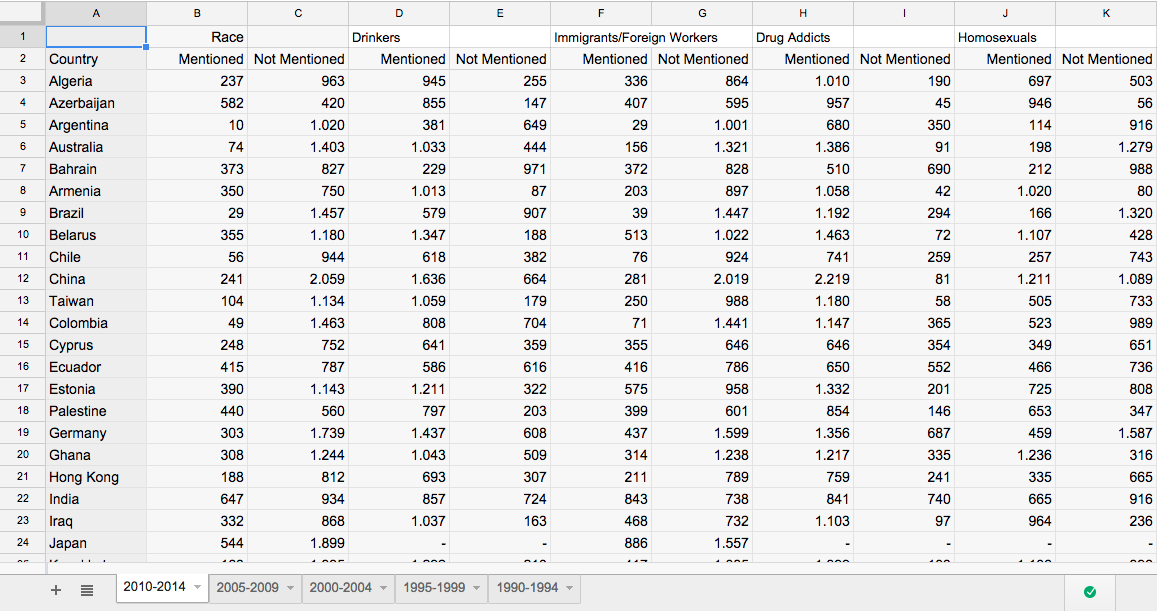
\includegraphics[width=12cm,angle=0]{tabdata1.png}
}
\caption{\label{tab1}}
\end{figure}

Then I proceeded in encoding this data to a JSON-style format that could be read by the web app(fig.~\ref{json}).
\begin{figure}[H]
\centering
{
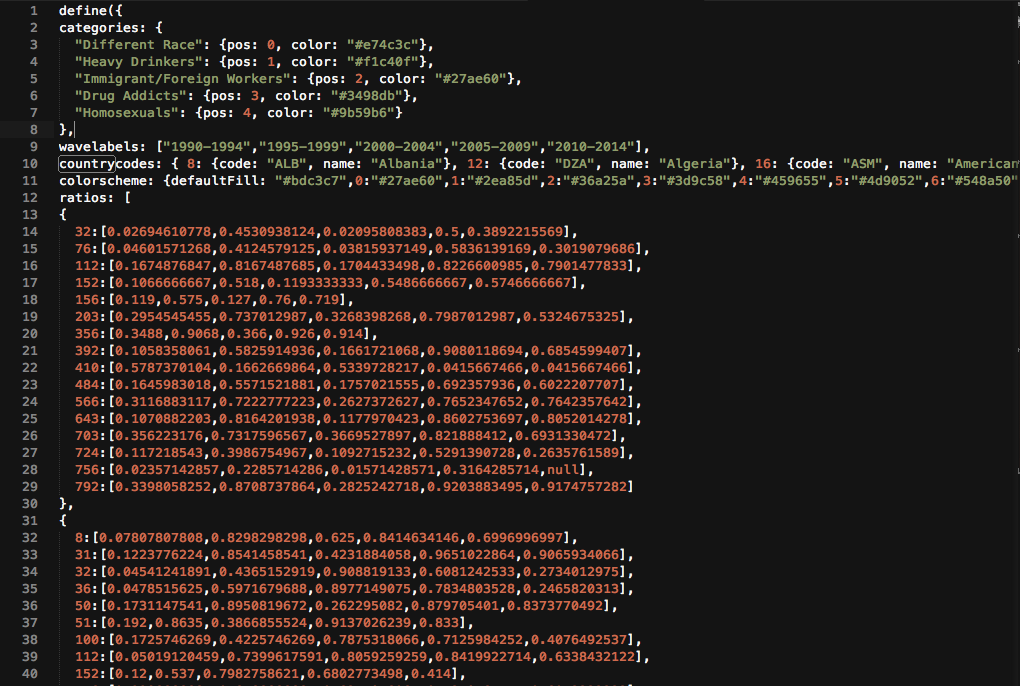
\includegraphics[width=12cm,angle=0]{json2.png}
}
\caption{\label{json}}
\end{figure}
\begin{figure}[h]
\centering
{
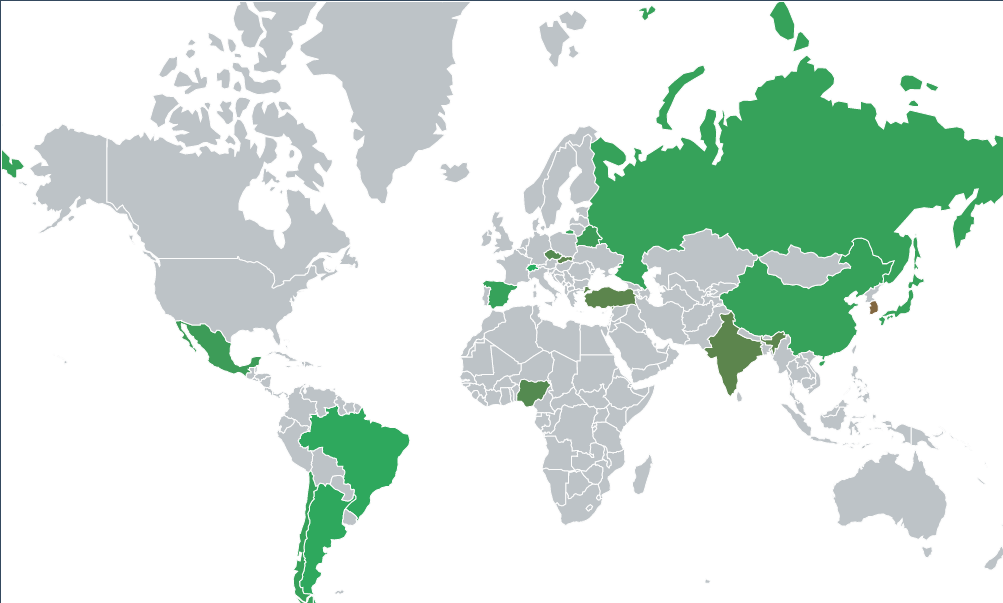
\includegraphics[width=12cm,angle=0]{map1.png}
}
\caption{\label{map1}}
\end{figure}
\paragraph{Coding} Now for the webpage.
First thing was to learn my way around D3. After a little playing around I finally loaded a map (fig.~\ref{map1}) and color the countries with different colors. Yay!
Decided that a mercator projection was the easiest for the user to select states in Europe, sorry map geeks.
\begin{figure}[h]
\centering
{
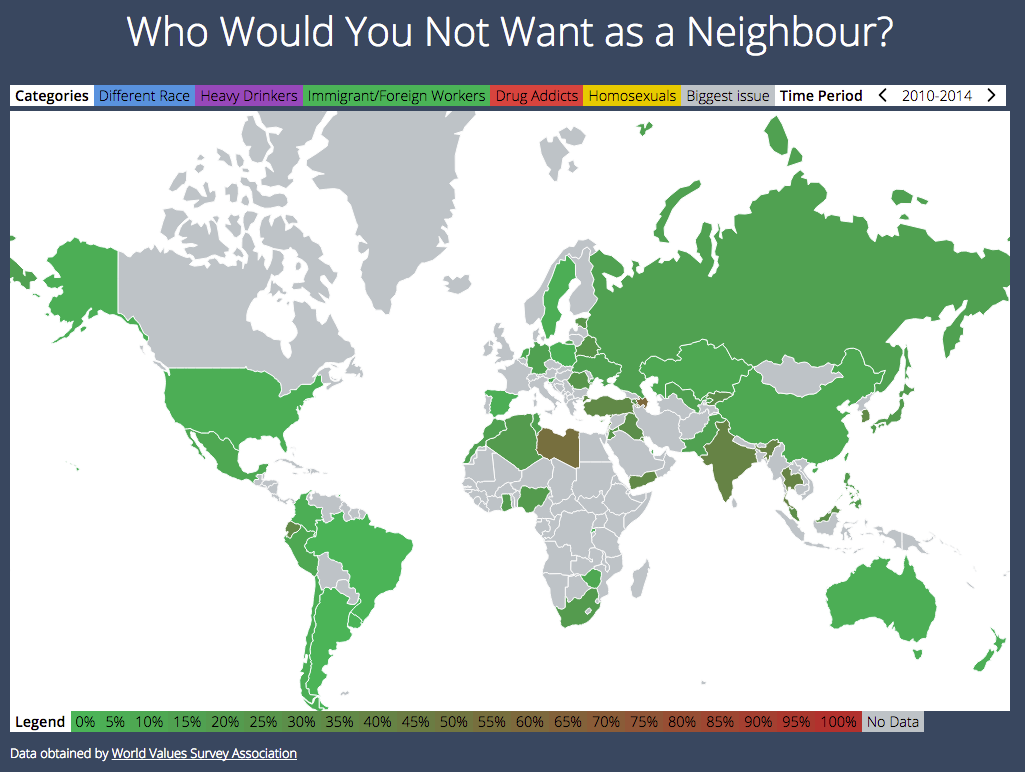
\includegraphics[width=12cm,angle=0]{map2.png}
}
\caption{\label{map2}}
\end{figure}

Now for adding some interaction: a control bar was added to change between the different categories and change the time period(fig.~\ref{map2}). 

\begin{figure}[h]
\centering
{
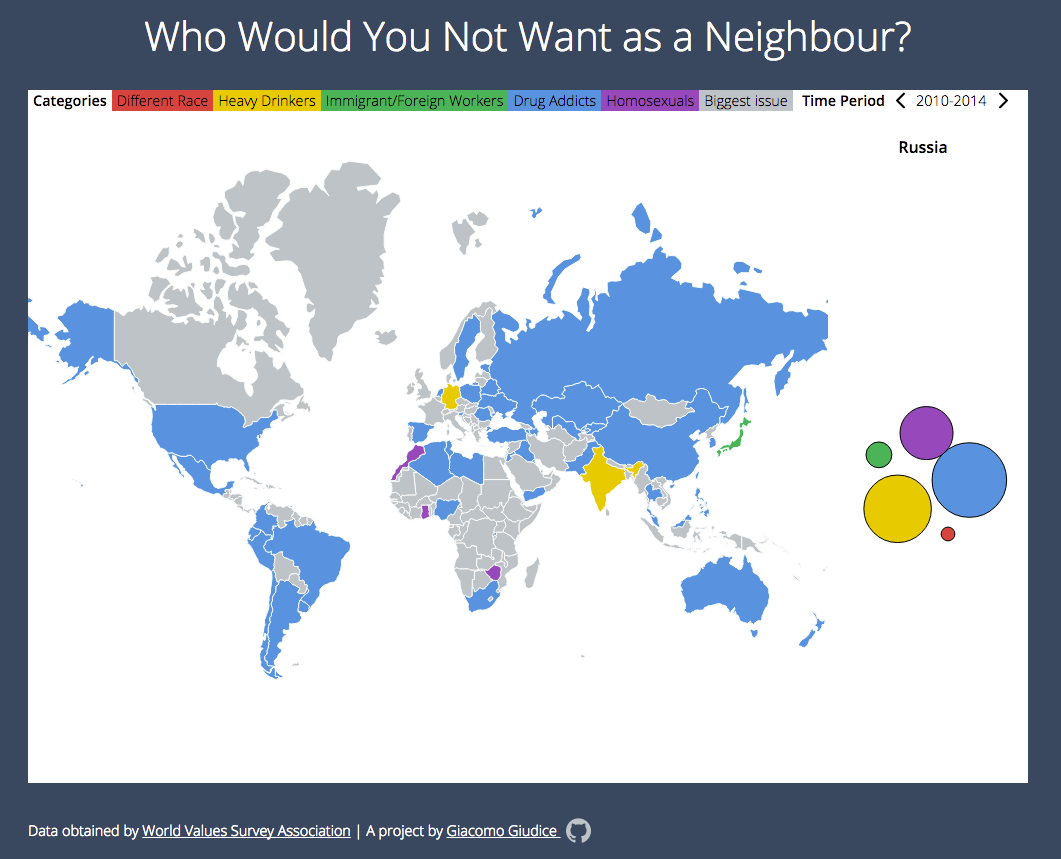
\includegraphics[width=12cm,angle=0]{map3.png}
}
\caption{\label{map3}}
\end{figure}
Finally the last feature added was a bubble chart depicting the size of each category when the user clicked on a country(fig.~\ref{map3}).
\end{document} %%%% THE END %%%%
